\section{Czym są grafy?}

Poniższy rysunek \ref{fig:road} przedstawia fragment mapy drogowej. 

\begin{figure}[H]
\centering
\includegraphics{road}
\caption{Fragment mapy drogowej \cite[11]{wilson}}
\label{fig:road}
\end{figure}

Możemy ją w uproszczeniu przedstawić za pomocą punktów i odcinków, tak jak na rysunku \ref{fig:road-graph}.

\begin{figure}[H]
\centering
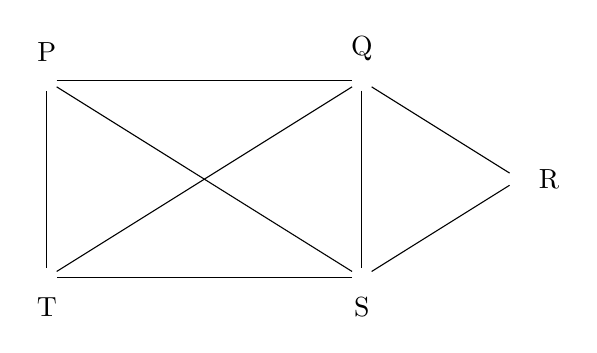
\begin{tikzpicture}
\filldraw 
(0,2.5) node[label=P](P){}
(4,2.5) node[label=Q](Q){} 
(6,1.25) node[label={right:R}](R){}
(4,0) node[label={below:S}](S){}
(0,0) node[label={below:T}](T){};
\path[draw] (P)--(Q);
\path[draw] (Q)--(R);
\path[draw] (R)--(S);
\path[draw] (S)--(T);
\path[draw] (T)--(P);
\path[draw] (P)--(S);
\path[draw] (Q)--(T);
\path[draw] (Q)--(S);
\end{tikzpicture}
\caption{Uproszczone przedstawienie fragmentu mapy drogowej} \label{fig:road-graph}
\end{figure}

Punkty $P,Q,R,S,T$ nazywamy \textbf{wierzchołkami}, odcinki nazywamy \textbf{krawędziami}, a cały wykres -- \textbf{grafem}. Punkt przecięcia odcinków $PS$ z $QT$ nie jest wierzchołkiem (nie odpowiada on skrzyżowaniu ulic).

Ten sam graf może modelować również inną sytuację. Przykładowo wierzchołkami mogą być osoby, a krawędź może oznaczać relację znajomości. Tak więc osoba $P$ zna osobę $T$, ale nie zna osoby $R$ (choć mają wspólnych znajomych $Q$ i $S$). 

Tę samą sytuację obrazuje także graf przedstawiony na rysunku \ref{fig:road-graph-alt}, w którym pozbyliśmy się przecięcia odcinków $PS$ i $QT$. Jednak nadal graf ten dostarcza informacji o tym, czy dane osoby znają się lub czy pomiędzy dwoma skrzyżowaniami istnieje bezpośrednia droga. Informacje, które tracimy dotyczą własności ,,metrycznych'' (takich jak długość\footnote{Choć tę informację możemy zachować, przypisując do każdej krawędzi \textbf{wagę}.} czy kształt drogi).  

\begin{figure}[H]
\centering
\begin{tikzpicture}
\filldraw 
(0,2.5) node[label=P](P){}
(4,2.5) node[label=Q](Q){} 
(6,1.25) node[label={right:R}](R){}
(4,0) node[label={below:S}](S){}
(0,0) node[label={below:T}](T){};
\path[draw] (P)--(Q);
\path[draw] (Q)--(R);
\path[draw] (R)--(S);
\path[draw] (S)--(T);
\path[draw] (T)--(P);
\path[draw] (P)--(S);
\path[draw] (Q)--(S);
\draw [-] (T) to [out=140,in=-120] (-0.4,2.9) to [out=60, in=140 ] (Q);
\end{tikzpicture}
\captionsetup{justification=centering}
\caption{Fragment mapy drogowej lub relacja znajomości narysowana bez ,,przecięć''} \label{fig:road-graph-alt}
\end{figure}

Tak więc graf przedstawia pewien zbiór punktów i dostarcza informacji, które z nich są ze sobą połączone. Oznacza to, że dwa grafy, które modelują tę samą sytuację, tak jak na rysunkach \ref{fig:road-graph} oraz \ref{fig:road-graph-alt}, są uznawane za identyczne \cite[12]{wilson} (niezależnie od sposobu w jaki narysujemy krawędzie oraz jak rozmieścimy wierzchołki). 

W tym miejscu warto również wspomnieć, że podobnie jak pomiędzy dwoma skrzyżowaniami lub miastami może istnieć wiele dróg, tak i w grafach dwa wierzchołki może łączyć więcej niż jedna krawędź (tzw. \textbf{krawędzie wielokrotne}). Inną analogią są drogi jednokierunkowe -- ich grafowym odpowiednikiem są \textbf{krawędzie skierowane}. 

Po tej wstępnej sekcji, która miała na celu zarysować czym są grafy, nastąpi sekcja zawierająca formalne definicje oraz pojawi się więcej pojęć związanych z teorią grafów. 